\documentclass[a4paper, 12pt]{report}

\usepackage[finnish]{babel}         % Suomenkielinen tavutus
\usepackage[fixlanguage]{babelbib}
\selectbiblanguage{finnish}
\usepackage[utf8]{inputenc}
\usepackage[T1]{fontenc}
\usepackage{ifpdf}
\usepackage{graphicx}
% load tocbibind package 
%   - do not include table of contents in itself
%   - convert the name of bibliography to references
\usepackage[nottoc]{tocbibind}

% load sverb package
%   - enhanced handling of verbatim stuff; listing environment
\usepackage{sverb}

% load listings package
%   - handle inclusion of source code
\usepackage{listings}
\usepackage{textcomp}
\usepackage{xcolor}

\usepackage{caption}
\usepackage{float}
\usepackage{setspace}
\captionsetup{font={small,stretch=1.1}}

\renewcommand{\lstlistingname}{Listaus}
\lstset{upquote=true,mathescape=false}

% Define JS for listings package
% Source: https://gist.github.com/Geruhn/3d21f60a869457373d84
\definecolor{lightgray}{RGB}{247, 247, 247}
\definecolor{darkgreen}{rgb}{0.0, 0.5, 0.0}
\definecolor{keyword_blue}{HTML}{0141CB}
\lstdefinelanguage{JavaScript}{
  keywords={
    any, do, if, for, let, new, try, var, case, else, enum, eval, null, this,
    true, void, with, await, break, catch, class, const, false, super, throw,
    while, yield, delete, export, import, public, return, static, switch,
    typeof, default, extends, finally, package, private, continue, debugger,
    function, arguments, interface, protected, implements, instanceof, type,
    of
  },
  morecomment=[l]{//},
  morecomment=[s]{/*}{*/},
  morestring=[b]',
  morestring=[b]",
  ndkeywords={class, export, boolean, throw, implements, import, this},
  keywordstyle=\color{keyword_blue}\bfseries,
  ndkeywordstyle=\color{darkgray}\bfseries,
  identifierstyle=\color{black},
  commentstyle=\color{darkgreen}\ttfamily,
  stringstyle=\color{red}\ttfamily,
  sensitive=true,
}

\lstset{
   language=JavaScript,
   backgroundcolor=\color{lightgray},
   extendedchars=true,
   basicstyle=\linespread{1.1}\footnotesize\ttfamily,
   aboveskip={15pt},
   showstringspaces=false,
   showspaces=false,
   numbers=left,
   numberstyle=\footnotesize,
   numbersep=9pt,
   tabsize=2,
   breaklines=true,
   showtabs=false,
   captionpos=b,
   literate={\$}{{{\$}}}1 {ä}{{\"a}}1 {Ä}{{\"A}}1 {ö}{{\"o}}1 {Ö}{{\"O}}1,
   frame=single
}

% Never insert line breaks in these words:
\hyphenation{JavaScript}
\hyphenation{EcmaScript}
\hyphenation{EcmaScriptin}
\hyphenation{JavaScriptille}
\hyphenation{JavaScriptillä}
\hyphenation{JavaScriptin}
\hyphenation{Closure}
\hyphenation{TypeScript}
\hyphenation{TypeScriptiä}
\hyphenation{Flow}
\hyphenation{tyypittäminen}
\hyphenation{stan-dar-din}
\hyphenation{VSCode}
\hyphenation{debugattaessa}

% load fancyheaders package
%   - the actual headers and footers are set later
\usepackage{fancyhdr}

% load itpackage 
%   - additional defines and stuff
\usepackage{thesis/itpackage}

\usepackage{enumitem}

\PassOptionsToPackage{hyphens}{url}\usepackage{hyperref}

% Command for inline code, like markdown `code`
\newcommand{\inlinecode}[1]{\colorbox{lightgray}{\texttt{#1}}}

\newcommand{\dblquoted}[1]{\textquotedbl#1\textquotedbl}

\title{JavaScriptin staattinen tyypittäminen}
\author{Oskari Noppa \\kandidaatintutkielma \\ tietojenkäsittelytiede \\ Turun yliopisto}
\date{Toukokuu 2019}

\begin{document}
  \selectlanguage{finnish}\fintrue

  \iffin
  \settocbibname{Lähdeluettelo}
  \renewcommand{\appname}{Liitteet}
  \else
  \settocbibname{References}
  \renewcommand{\appname}{Appendices}
  \fi
  
  % Fill in your information below
  \workinfo{Oskari Noppa}
  {JavaScriptin staattinen tyypittäminen}
  {Jari-Matti Mäkelä}
  {Second Supervisor}
  {2019}
  {5}
  {Toukokuu}
  
  % Set the type of your thesis (Diplomityö, TkK -tutkielma, etc.) and
  % laboratory or field of study below
  \worktype{}{LuK -tutkielma} 
  \deptinfo{}{Tietojenkäsittelytiede}
  
  % Generate the title page 
  \gentitle
  % empty pagestyle for table of contents etc. 
  %
  % the redefinition of plain style works also for 1st pages of chapters,
  % which is the default in report class. Just state \thispagestyle{empty}
  % after \chapter{something} if you want empty style for the 1st pages. 
  %
  \pagestyle{empty}
  \fancypagestyle{plain}{
    \fancyhf{}
    \renewcommand{\headrulewidth}{0 pt}
  }
  
  % roman numbering for table of contents etc.
  \pagenumbering{roman}
  
  % insert table of contents, list of figures, list of tables
  %
  % setting the counter to zero effectively removes the page number from
  % the toc, lof etc. entries in the toc since there is no roman numeral
  % for zero ;-) (if you want them without numbering)
  %
  %\setcounter{page}{0}

  \begin{ittiivis}{JavaScript, tyyppijärjestelmä, TypeScript, Flow, Closure}
Tässä tutkielmassa tutustutaan kolmeen JavaScript-ohjelmointikieltä
täydentävään työkaluun, jotka lisäävät dynaamisesti tyyppitarkastettuun
JavaScriptiin staattisen tyyppitarkastuksen. JavaScriptillä kehitettävien
ohjelmistojen määrä ja kompleksisuus on kasvanut suuremmaksi kuin mihin
JavaScript oli alkujaan tarkoitettu, mikä voi aiheuttaa ohjelmiston
laatuun ja koodin ylläpidettävyyteen liittyviä ongelmia.
TypeScript, Flow ja Closure-kääntäjä analysoivat JavaScript-koodia sekä
siihen lisättäviä tyyppiannotaatioita ja voivat auttaa ohjelmiston kehittäjää
välttämään näitä ongelmia.

Tutkielmassa näytetään kuinka käännösaikana tehtävä staattinen tyyppitarkastus
voi parantaa ohjelmistojen toimivuutta ja ylläpidettävyyttä verrattuna
dynaamiseen tyyppitarkastukseen yleisesti, sekä esitellään tapoja joilla
erityisesti JavaScript-ohjelmistoja voidaan optimoida käännösaikana
staattisen tyyppijärjestelmän avulla. TypeScriptin, Flow'n ja Closuren
käyttöönottoa ja käyttöä vertaillaan myös toisiinsa, alkaen siitä kuinka
JavaScriptillä kirjoitettu ohjelmistoprojekti voidaan muuttaa staattisesti
tyyppitarkastetuksi kutakin työkalua käyttäen.

Lopuksi tarkastellaan JavaScriptilla kirjoitettujen ohjelmien staattisessa
tyypittämisessä vastaan tulevia ongelmia, sekä niitä valintoja joita
tutkielmassa esiteltyjen työkalujen suunnittelussa on tehty hyötyjen
ja haittojen tasapainottamiseksi.
  \end{ittiivis}
  

  \tableofcontents
  \clearpage
  %\setcounter{page}{0}
  %\listoffigures 
  %\clearpage
  %\setcounter{page}{0}
  %\listoftables
  
  % possibly insert 'list of acronyms'
  %
  %   - create a chapter called List Of Acronyms (or whatever), which
  %     should contain all your acronym definitions, e.g. 
  %     \chapter{List Of Acronyms} 
  %   - the secnumdepth trickery is needed because acronyms are as a
  %     standard chapter and we are faking '\listofacronyms'
  %
  %\setcounter{secnumdepth}{-1}
  %\input{your acronym chapter's file name}
  %\setcounter{secnumdepth}{2}
  
  % setup page numbering, page counter, etc.
  \startpages

  \chapter{Johdanto} \label{Johdanto}

Ohjelmointi on pohjimmiltaan tietorakenteiden käsittelyä ja yksi tärkeimmistä
tietorakenteen ominaisuuksista on sen tyyppi. Muuttuja \dblquoted{nimi} voi olla
datatyypiltään teksti ja muuttuja \dblquoted{ikä} voi olla numero, eikä näitä kahta voi
huolettomasti sekoittaa. Ohjelman tila ei ole järkevä jos se sanoo henkilön
iän olevan \dblquoted{Matti}. Se miten ohjelmointikielissä käsitellään arvojen tyyppejä
vaihtelee kuitenkin suuresti.

Tässä tutkielmassa käsitellään JavaScriptiä, sekä kolmea työkalua jotka
rakentavat staattisesti tarkastettavan tyyppijärjestelmän
JavaScriptin päälle. JavaScript on \textit{dynaamisesti tyypitetty} ohjelmointikieli,
jonka alkuperäinen käyttötarkoitus oli lisätä verkkosivuille pieniä
interaktiivisia ominaisuuksia, kuten lomakkeiden validointia. JavaScriptillä
toteutettavien ohjelmien koko, monimutkaisuus ja tärkeys on kuitenkin viime
vuosien aikana kasvanut alkuperäistä tarkoitusperää suuremmaksi, kun sillä on
alettu toteuttaa esimerkiksi kartta-, kirjoitus- ja hallintapalveluita jotka
toimivat selaimessa, siten ettei käyttäjän tarvitse asentaa erillistä
tietokoneohjelmaa palvelun käyttöön. JavaScriptia on myös alettu käyttää
verkkosivujen \textit{front-end} käyt\-tö\-liit\-ty\-mä\-to\-teu\-tuk\-sen
lisäksi tietokone- ja kän\-nyk\-kä\-so\-vel\-luk\-sis\-sa, sekä
pal\-ve\-lin\-kie\-le\-nä \textit{back-endillä}.

Tutkielmassa esitellään TypeScript, Flow ja Closure-kääntäjä, joista jokainen on
tarkoitettu työkaluksi sellaisten ohjelmien kehittämiseen,
jotka muuten kehitettäisiin\newline
JavaScriptilla. Päämääränä on esitellä kuinka dynaamisesti
tyypitetty JavaScript voidaan muuttaa staattisesti tyyppitarkastetuksi
TypeScriptin, Flown, tai Closure-kääntäjän avulla, sekä mitä hyötyä siitä voi
olla. Työkalujen hyötyjä ja haittoja vertaillaan sekä toisiinsa että
tavalliseen JavaScript-koodiin.

  \section{Peruskäsitteitä}
\subsection{Määritelmiä}

On hyvä huomioida ero termien välillä kun puhutaan staattisesta ja
%                                       "heikko" = "löyhä"?
dynaamisesta, tai toisaalta vahvasta ja heikosta tyypittämisestä. Myös
dynaamisesti tyypitetty kieli voi nostaa virheen väärien tietotyyppien
käyttämisestä ohjelman suorittamisen aikana, etenkin jos se on vahvasti
tyypitetty kieli. Tässä tutkielmassa keskitytään kuitenkin lähinnä
staattiseen ja dynaamiseen tyypitykseen, eli siihen miten tietotyyppeihin
liittyviä virheitä käsitellään käännös aikana, jo ennen ohjelman
suorittamista.
  \chapter{JavaScript-ohjelman muuttaminen staattisesti tyyppitarkastetuksi}

\section{Tyyppiannotaatiot}

Tyyppijärjestelmä voi päätellä muuttujan sallitun tyypin automaattisesti
päättelemällä tai kieleen sisältyvien eksplisiittisten tyyppimäärittelyjen
perusteella. Kaikki kolme tässä tutkielmassa esiteltyä JavaScriptin staattiseen
tyyppitarkastukseen tarkoitettua työkalua päättelevät muuttujien tyyppejä automaattisesti,
mutta vaativat paikoitellen myös eksplisiittisiä määrityksiä.
Closure-kääntäjä lukee
tyyppimääritykset JSDoc-tyylisistä dokumentaatiokommenteista \cite{annotatingJSforClosure}.
\begin{lstlisting}[caption={Esimerkki Closure-annotaatiosta funktiolle},label={lst:ostoskorin_hinta_closure}]
/**
* @param {!Array<Ostos>} ostokset
* @return {number} Ostosten yhteenlaskettu hinta
*/
function ostoskorinHinta(ostokset) {
  let summa = 0;
  for (const ostos of ostokset) summa += ostos.hinta;
  return summa;
}
\end{lstlisting}
Listauksessa \ref{lst:ostoskorin_hinta_closure} \inlinecode{ostoskorinHinta}-funktion
tyyppimäärittely on toteutettu sen yläpuolella olevilla kommenteilla, jotka määrittävät
tyypin \inlinecode{ostokset} parametrille sekä funktion palautusarvolle.
TypeScript ja Flow puolestaan jatkavat ECMA-262 -spesifikaatiota erityisellä syntaksilla
tyyppien eksplisiittistä määrittämistä varten. 
\begin{lstlisting}[
  float,
  caption={Esimerkki Flow tai TypeScript annotaatiosta funktiolle},
  label={lst:ostoskorin_hinta_flow}
]
function ostoskorinHinta(ostokset: Ostos[]): number {
\end{lstlisting}
Flow ja TypeScript -esimerkeissä \ref{lst:ostoskorin_hinta_flow}
tyyppiannotaatiot ovat osana koodia, mikä
tekee ohjelmasta yhteensopimattoman tavallisen JavaScriptin kanssa. Ohjelma
on käännettävä JavaScriptiksi ennen suorittamista. Annotaatioiden
syntaksi ja merkitys ei myöskään ole välttämättä suoraan selvä
JavaScript-ohjelmoijalle, joka pahimmassa tapauksessa voi kokea lisätyt
tyyppimäärittelyt vaikeasti luettavina. 

Closuren annotaatiot on sijoitettu kommentteihin, joten niillä ei ole
ajonaikaista vaikutusta ja ohjelma on täten sellaisenaan hyväksyttävää
JavaScriptiä. Toisaalta tyyppiannotaatioiden määrittely kommenteissa voi
olla runsassanaista ja hankalaa, mikä kasvattaa niiden kirjoittamiseen vaadittua
työmäärää \cite{TypeScriptSpec, TypeScriptatBuild}.

Aiemmassa esimerkissä esitelty tyyppi \inlinecode{Ostos} pitäisi
määritellä Closurea varten muiden annotaatioiden tapaan dokumentaatiokommentteja käyttäen:

\begin{lstlisting}[label={lst:closure_typedef}]
/**
* @typedef {{
*   nimi: string,
*   hinta: number
* }}
*/
let Ostos;
\end{lstlisting}
TypeScript ja Flow tarjoavat käännösaikaisen tyypin (type alias)
määrittelyyn tiiviimmän ja helppolukuisemman syntaksin \cite{TypeScriptSpec}:
\begin{lstlisting}[label={lst:ts_flow_type_alias}]
type Ostos = {
  nimi: string;
  hinta: number;
};
\end{lstlisting}
Tällainen tyypin määritteleminen vaikuttaa ainoastaan käännösvaiheen
tyyppitarkastukseen, eikä määrittely tuota tietorakenteita tai muuta
sisältöä suoritettavaan JavaScript-ohjelmaan.

\section{Ohjelman kääntäminen ennen suorittamista}
\begin{figure}[!htb]
\centering
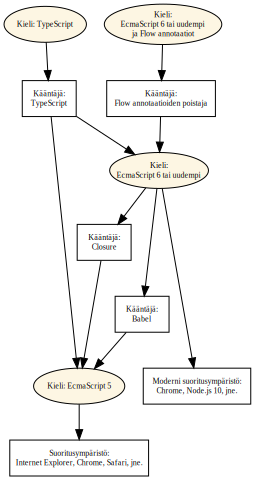
\includegraphics[width=0.6\textwidth]{images/compilation.pdf}
\caption{Vaihtoehtoisia käännösprosesseja}
\label{fig:compilation}
\end{figure}
JavaScript-koodi tulkataan tai käännetään tyypillisesti suorittamisen
yhteydessä, selaimesta tai muusta suoritusympäristöstä löytyvän ”moottorin”
toimesta. EcmaScript-standardin mukaista koodia suorittamaan suunnitellut
moottorit, kuten V8 tai SpiderMonkey, eivät kuitenkaan osaa käsitellä
TypeScript- tai Flow-annotaatioilla merkattua koodia. Näinollen TypeScript-
tai Flow-annotoitu koodi on välttämätöntä kääntää muotoon jossa
annotaatiot on poistettu ja jäljellä on enää standardinmukainen JavaScript.
Koska JavaScriptin käyttäminen ei normaalisti vaadi erillistä
käännösvaihetta, useissa projekteissa ei ole sellaista käytetty. Koodin
minimointi ja muu optimointi on ollut parhaiden käytäntöjen mukaista jo
tovin, mutta tällaiset koodinkäsittelyt tehdään yleensä vasta ennen ohjelman
julkaisua. Kehittäjät ovat tavanomaisesti voineet suorittaa kirjoittamansa
JavaScriptin sellaisenaan kehitysympäristössä. Käännösvaiheen aikavaatimus
pyritään luonnollisesti pitämään mahdollisimman pienenä, mutta se on silti
projektin monimutkaisuuteen ja kehitysnopeuteen vaikuttava tekijä, joka
tulee huomioida työkalun käyttöönotossa.

Kuva \ref{fig:compilation} esittää erilaisia käännösprosesseja eri
JavaScript-ohjelman kehityskielille. Jos koodi kirjoitetaan kaikkiin
suoritusympäristöihin soveltuvalla kielen versiolla, kuten EcmaScriptin
versiolla 5 (2011), käännösvaihe voidaan jättää kokonaan väliin. Kielen
uudemmat versiot ovat kuitenkin tuoneet monia lisäominaisuuksia, joiden
käyttäminen vanhempia selaimia tukevissa ohjelmissa vaatii joka tapauksessa
käännösvaiheen staattisesta tyypittämisestä riippumatta. Uusia JavaScript-
ominaisuuksia hyödyntäville projekteille koodin kääntäminen ei siis tule
täysin uutena vaiheena.

\section{Työkalun vaiheittainen käyttöönotto}

JavaScript-kirjastojen hallintaan tarkoitettu rekisteri npm on yksi
suurimmista ohjelmistoekosysteemeistä \cite{DynamicsOfJSPackages}.
Tutkinnon kirjoittamisen hetkellä rekisterin kotisivu, npmjs.com ilmoitti
ladattavissa olevien pakettien määräksi yli 800 000. Avoimessa jakelussa
olevien kirjastojen lisäksi JavaScriptiä käyttävillä kehittäjillä voi olla
suuri määrä valmista JavaScript-koodia, jota voi hyödyntää uusissa
projekteissa. Jotta TypeScript, Flow ja Closure olisivat hyödyllisiä
työkaluja JavaScript-ohjelmien kehitykseen, on niiden oltava yhteensopivia
sellaisen JavaScript-koodin kanssa jonka kehitykseen ei kyseistä työkalua
ole käytetty.

TypeScript ja Flow tukevat erityisiä määrittelytiedostoja, joiden sisältämällä
tyyppiannotoidulla koodilla määritetään kirjaston tai muun JavaScript-koodin
ulkoisen rajapinnan tyyppimäärittelyt. Näiden tiedostojen kirjoittamiseen
käytetty syntaksi on muuten sama kuin muissakin tiedostoissa, muuta niiden funktio- ja
metodimäärittelyistä on jätetty implementaatiot kokonaan pois. Tiedoston ei
ole tarkoitus olla osana varsinaista suoritettavaa koodia, vaan se palvelee
ainoastaan kuvauksena sellaisen koodin tyyppimäärittelystä, jonka käsittelyä
TypeScript ja Flow eivät muuten voisi valvoa. TypeScriptillä voitaisiin
esimerkiksi kirjoittaa seuraava tiedosto \inlinecode{ostoskori.d.ts}, jonka
tehtävä on annotoida toista tiedostoa \inlinecode{ostoskori.js}.
\begin{lstlisting}[caption={Esimerkki TypeScript määrittelytiedostosta ostoskori.d.ts}]
export const tuotteet: ReadonlyArray<Ostos>;

/** Lisää tuotteen ostoskoriin. */
export function lisääTuote(ostos: Ostos): void;
\end{lstlisting}
Tämän jälkeen TypeScript tiedostosta käsin voidaan kutsua tätä
JavaScript-funktiota siten, että TypeScript valvoo
tyyppien oikeellisuutta.
\begin{lstlisting}[caption={JavaScript-koodin kutsuminen TypeScript tiedostosta tuotesivu.ts}]
import * as ostoskori from "./ostoskori";

ostoskori.lisääTuote({ nimi: "juusto", hinta: 5 });
// Vääränlainen kutsumistapa aiheuttaisi käännösaikaisen virheen:
// ostoskori.lisääTuote('juusto', 5);
\end{lstlisting}

Joissain tapauksissa kirjastoille tai kehittäjän omalle aiemmin kirjoitetulle
JavaScript-koodille ei kuitenkaan ole valmiita TypeScript-tyyppimäärittelyjä
eikä niitä syystä tai toisesta voida luoda ennen muun kehityksen jatkamista.
Kaikkien kolmen työkalun tärkeimpiin ominaisuuksiin kuuluu tuki vaiheittaiselle
käyttöönotolle, eli käytännössä yhteenspivuus täysin tyyppitarkastamattoman
koodin kanssa. Sekä Flow että TypeScript tarjoavat erityisen
yleisviittaustyypin Any, jota voi käyttää kuvaamaan mitä tahansa JavaScript
arvoa \cite{TypeScriptSpec}. Any-tyyppiseen muuttujaan voidaan asettaa mikä
tahansa arvo ja Any tyyppinen arvo voidaan asettaa mihin tahansa muuttujaan
tai funktioparametriin. Any tyypin avulla muuten staattisesti tyypitetyssä
ohjelmassa voidaan ohittaa käännösaikainen tyyppien tarkistaminen sellaisten
koodin osien kohdalla joiden ajonaikaista arvoa olisi muuten vaikea tai
mahdotonta määritellä käännösaikana. Näin ollen, mikäli tarve vaatii täysin
annotoimattoman JavaScript moduulin käyttämistä, kaikkien kyseisestä moduulista
tuotujen arvojen voidaan määrittää olevan tyyppiä Any, jolloin tarkastaja ei
kiinnitä huomiota siihen miten JavaScriptillä määritettyjä funktioita tai
muita arvoja käsitellään.
  \chapter{Virheiden havaitseminen}

\section{Virheiden havaitseminen}

Kenties tärkein staattisen tyyppijärjestelmän tehtävä on havaita ja estää
ohjelmoijan virheitä. Tässä esitellyt työkalut, mahdollisesti Closure
kääntäjää lukuunottamatta, onkin kehitetty erityisesti tätä tarkoitusta
varten.

Kaikki kolme työkalua antaisivat käännösvirheen jos esimerkeissä
\ref{lst:ostoskorin_hinta_clojure} ja \ref{lst:ostoskorin_hinta_flow}
esiteltyä funktiota kutsuttaisiin virheellisesti esimerkiksi listalla
hintaa kuvaavia numeroita, sillä funktion parametrin on annotoitu olevan
lista ``Ostos''-tyyppimääritelmän mukaisia objekteja. Esimerkiksi
virheellinen kutsu
\colorbox{lightgray}{\lstinline|ostoskorinHinta([5, 10, 15])|} ei itse
asiassa aiheuttaisi suoritettaessa ohjelman keskeyttävää virhettä.
\colorbox{lightgray}{\lstinline|ostos.hinta|} ilmaisu on sallittu vaikka
muuttuja \colorbox{lightgray}{\lstinline|ostos|} olisikin arvoltaan numero
eikä objekti. Tällöin ilmaisun arvo on \colorbox{lightgray}{\lstinline|undefined|}
ja lausekkeen \colorbox{lightgray}{\lstinline|summa += ostos.hinta|} jälkeen
\colorbox{lightgray}{\lstinline|summa|} muuttujan arvo on erityinen
ei-numeroa kuvaava \colorbox{lightgray}{\lstinline|NaN|} \cite{Ecma262NaN}.
Käännösaikaisen tarkistamisen merkitys korostuu erityisen hyödylliseksi
tämänkaltaisen ohjelmointivirheen kohdalla, sillä virhe ei välttämättä ole
muutoin helposti havaittavissa. Funktiokutsu ei aiheuttaisi helposti
todennettavaa suoritusaikaista virhettä, joten ei-toivottu palautusarvo
\colorbox{lightgray}{\lstinline|NaN|} saattaisi kiertää ohjelman
operaatioiden välillä pitkällekin aiheuttaen muita loogisia virheitä.

Vuonna 2017 tehdyssä tutkimuksessa TypeScriptin ja Flown vaikutuksesta avoimen
lähdekoodin JavaScript-projekteihin havaittiin, että vähintään 15\%
ilmoitetuista ja korjatuista bugeista olisi voitu havaita ja välttää jos
projektin kehitykseen oltaisin käytetty jompaakumpaa näistä työkaluista \cite{ToTypeOrNotToType}.
Tutkimuksen arvioinnissa huomioitiin lisäksi, että tulos on tutkimusmenetelmästä
johtuen mitä luultavimmin alempi kuin tällaisen muutoksen tuoma todellinen
vaikutus.

\section{Ohjelman optimointi käännösvaiheessa}
TODO

\section{Tyyppimäärittelyt dokumentaationa}
TODO
  \chapter{Ongelmat JavaScriptin staattisessa tyypittämisessä}

\section{EcmaScript-yhteensopivuus}
TypeScript pyrkii noudattamaan EcmaScript-spesifikaatiota mahdollisimman
tarkasti kaikkien sellaisten ominaisuuksien suhteen jotka eivät nimenomaan
liity staattiseen tyypittämiseen \cite{TypeScript_DesignGoals}. TypeScriptin
kehityksen alkuvaiheissa, ennen EcmaScript 2015-spesifikaation valmistumista,
JavaScriptista kuitenkin puuttui joitain tärkeiksi katsottuja ominaisuuksia,
jotka päätettiin lisätätä TypeScriptiin mahdollisista yhteensopimusongelmista
huolimatta. TypeScriptissä on esimerkiksi syntaksi nimiavaruuden määrittämiseen,
vaikka EcmaScriptiin myöhemmin lisätyt \textit{moduulit} ajavat saman asian
\cite{TypeScript_issuecomment_esnextfeatures}. TypeScript tukee nykyään sekä
alkuperäistä nimiavaruus-ominaisuuttaan että EcmaScriptin moduuleita.

Flow ja Closure-kääntäjä lisäävät koodiin ainoastaan staattista tyypitystä
koskevia ominaisuuksia, kuten tyyppimäärittelyjä, joten niissä ei ole
nimiavaruuksien kaltaisia koodin suoritukseen vaikuttavia ominaisuuksia.
EcmaScript kuitenkin kehittyy nopeasti ja sen päälle rakentavien työkalujen
on pysyttävä tahdissa mukana ollakseen hyödyllisiä kehittäjille.

Kaikki kolme työkalua pyrkivät tukemaan EcmaScriptin uusinta viimeisteltyä
versiota. Lisäksi Flow tarjoaa tyyppitarkastusta joillekkin kokeellisille
ominaisuuksille joiden EcmaScript-määrittely ei vielä ole täysin valmis mutta
jotka luultavasti tullaan lisäämään myöhemmin. Esimerkiksi
\textit{optional chaining} \cite{Optional_Chaining_proposal} on vielä
suunnitteluvaiheessa oleva kielen ominaisuus, mutta Flow tarjoaa jo
staattisen tyyppitarkastuksen sille. Uusien ominaisuuksien aikaisessa
käyttöönotossa on JavaScriptin kehityksen kannalta se hyvä puoli, että
kehittäjäyhteisö pääsee kokeilemaan ja antamaan palautetta ennen kuin ominaisuuden
määrittely on lyöty lukkoon. TypeScript puolestaan pyrkii vastedes implementoimaan
ainoastaan valmiita ominaisuuksia, sillä keskeneräisen ominaisuuden yksityiskohdat
tulevat suurella todennäköisyydellä muuttumaan useaan otteeseen suunnitteluvaiheen
aikana ja sitä käyttäneet kehittäjät voivat myöhemmin joutua
\textit{refaktoroimaan} koodiaan.

\section{Tyyppien automaattinen ja vaiheittainen tyypittäminen}

Todo

\section{Luotettavuus, täydellisyys ja käytännöllisyys}

\begin{figure}
\includegraphics[width=\textwidth]{images/soundness_completeness2.pdf}
\caption{Tyyppijärjestelmän luotettavuus ja täydellisyys}
\end{figure}

Tyyppijärjestelmän luotettavuus (soundness) kuvaa sitä, kuinka suuren osan
mahdollisista ohjelmointivirheistä se estää. Täysin luotettava (sound)
tyyppijärjestelmä estää kaikki sellaiset virheet jotka sen on tarkoitus
estää \cite{CSE_ProgrammingLanguages}. Täydellisyys (completeness)
puolestaan kertoo salliiko tyyppijärjestelmä kielen sellaiset ominaisuudet
jotka eivät olisi ajonaikana tyyppivirheitä \cite{TypesAndProgrammingLanguages, CSE_ProgrammingLanguages}.

Jotta JavaScriptiä analysoiva tyyppijärjestelmä olisi luotettava, sen on
annettava virhe esimerkiksi seuraavasta ohjelmasta:

\begin{minipage}{\linewidth}
\begin{lstlisting}[caption={Virheellinen JavaScript-ohjelma: Lisätyllä tuotteella ei ole nimeä.}]
function osta(ostos) {
  lisaaTuote({
    nimi: ostos.nimi,
    hinta: ostos.hinta
  });
}

osta({ nimi: 'juusto', hinta: 5 });
osta({ hinta: 5 });
\end{lstlisting}
\label{fig:soundness_test}
\end{minipage}

Toisaalta jotta JavaScriptiä analysoiva tyyppijärjestelmä olisi täydellinen,
sen on sallittava tämä korjattu versio ylläolevasta ohjelmasta:

\begin{minipage}{\linewidth}
\begin{lstlisting}[caption={Toimiva JavaScript-ohjelma: Virheelliseltä kutsulta on suojauduttu tarkistuksella.}]
function osta(ostos) {
  if (typeof ostos.nimi === 'string') {
    lisaaTuote({
      nimi: ostos.nimi,
      hinta: ostos.hinta
    });
  }
}

osta({ nimi: 'juusto', hinta: 5 });
osta({ hinta: 5 });
\end{lstlisting}
\label{fig:completeness_test}
\end{minipage}

Esimerkit \ref{fig:soundness_test} ja \ref{fig:completeness_test} toimivat
odotetulla tavalla Flow:ssa. TypeScript vaatii eksplisiittisen tyyppiannotaation
osta-funktiolle, mutta toimii muuten samalla tavalla. Flow, TypeScript ja
Closure eivät kuitenkaan ole täydellisiä tai kokonaan luotettavia.
Monimutkaisemmissa tilanteissa virheitä saattaa jäädä nappaamatta tai toimiva
ohjelma voidaan merkata virheelliseksi. JavaScriptiä käännöskohteena käyttävät
mutta muuten sen syntaksista ja semantiikasta eroavat uudet kielet,
kuten Dart ja Elm, on voitu kehittää toivotunlaiseksi ilman painetta olla
yhteensopiva vanhan koodin kanssa.

TypeScript ja Flow on sen sijaan kehitetty lisäämään staattinen tyypitys
olemassa olevaan kieleen, JavaScriptiin, siten että nykyisellään käytössä
olevat kirjastot ja koodikäytännöt pystytään tyyppitarkastamaan ilman että
niiden arkkitehtuuria tarvitsee merkittävästi muuttaa tyyppiturvallisuuden
saavuttamiskesi.

TypeScript on strukturaalisesti tyypitetty, minkä vuoksi seuraava koodi kääntyy
ilman tyyppivirheitä.

\begin{minipage}{\linewidth}
\begin{lstlisting}[caption={Loogisen virheen sisältävä, mutta ilman virheitä kääntyvä TypeScript-ohjelma.}]
class Ihminen {
    constructor(public nimi: string){}
}

class Elain {
    constructor(public nimi: string){}
}

function varaaAikaElainlaakariin(omistaja: Ihminen, lemmikki: Elain)
{
  ...
}

varaaAikaElainlaakariin(new Elain("Musti"), new Ihminen("Jaakko"));
\end{lstlisting}
\label{fig:structural_typing_error}
\end{minipage}

TypeScript-kääntäjä sallii esimerkin \ref{fig:structural_typing_error} koodin
vaikka arugmentit "omistaja" ja "lemmikki" ovat väärin päin, sillä
molempien luokkien rakenne on sama; molemmissa on pelkkä tekstimuotoinen
ominaisuus "nimi". Flow:ssa sama virhe ei menisi läpi. Siinä luokkainstanssit
on tyypitetty nominaalisesti, mikä auttaa tässä esimerkissä mutta aiehuttaa ongelmia
muissa tilanteissa. Projekti saattaa esimerkiksi sisältää kaksi versiota samasta
kirjastosta jonkin toisen kirjaston kautta, mikä voi aiheuttaa yhteensopimusongelmia
kun käytännössä saman luokan tyyppejä ei lueta keskenään yhteensopiviksi. 
  \chapter{Yhteenveto}
Staattinen tyypitys jakaa mielipiteitä. Facebook on kehittänyt
staattiset tyyppijärjestelmät myös \textit{Pythonin} (1990) ja \textit{PHP:n} (1995)
analysointiin \cite{PyreCheck, HackLang}.
Dynaamisesti tyypitetyn \textit{Clojuren} (2007) kehittäjä
Rich Hickey on puolestaan kritisoinut staattista
tyypitystä useaan otteeseen \cite{10YearsOfClojure}. Eksplisiittiset
tyyppimäärittelyt vaativat lisää kirjoitettavaa koodia ja liian tiukka
tyyppijärjestelmä voi rajoittaa sitä mitä kielellä voi tehdä, sillä harva
tyyppijärjestelmä on täydellinen (engl. complete). JavaScriptissä on useita
yleisesti käytettyjä rajapintoja jotka ovat hyödyllisiä mutta vaikeita
tyypittää staattisesti. Esimerkiksi suositusta kirjastosta \textit{lodash}
löytyy funktio \inlinecode{get} \cite{LodashGet}, jota voidaan kutsua
seuraavasti

\begin{lstlisting}[caption={
	get-funktiolla voidaan palauttaa arvo syvältä
	objektin sisältä välittämättä mahdollisesti puuttuvista arvoista.},
  label={fig:lodash_get_function},
  aboveskip={20pt}
]
	import {get} from 'lodash';

	const object = { a: [{ b: { c: 3 } }], d: null };
	get(object, 'a[0].b.c'); // Palauttaa numeron 3
\end{lstlisting}

Staattisen tyyppijärjestelmän on vaikea päätellä esimerkin get-kutsun
palautusarvo tai tarkistaa toisen argumentin oikeellisuus. Ohjelmoija joutuu
joko luopumaan tyyppiturvallisuudesta tässä
osassa koodia tai kirjoittamaan jonkin
huomattavasti monimutkaisemman version säilyttääkseen tyyppiturvallisuuden.

Dynaamisen koodin nopeasta kirjoitustahdista saatavat hyödyt jäävät kuitenkin
vähäisiksi jos lopputuotos ei toimi odotetulla tavalla. Bugit heikentävät
käyttäjien tyytyväisyyttä ohjelmaan ja voivat pahimmillaan aiheuttaa sellaista
vahinkoa että koko bugisen ohjelman julkaisusta saatu nettohyöty on negatiivinen,
eli sen käyttöönotto aiheuttaa enemmän haittaa kuin hyötyä. Staattinen tyypitys
ohjaa kirjoitettua koodia turvalliseen suuntaan kehitysvaiheen alusta
loppuun, ja torjuu tietynlaisia ohjelmointivirheitä tehokkaammin kuin
esimerkiksi ajonaikaista käyttäytymistä testaavat \textit{unit testit}.
Esimerkissä \ref{fig:lodash_get_function} esitelty get-kutsu on yksinkertainen
ja helppolukuinen, mutta jos muuttujan \inlinecode{object} tyyppiä myöhemmin
muutetaan toiseen muotoon muistamatta päivittää myös get-kutsua, virheellisestä
get-kutsusta voi muodostua ohjelmaan hankala bugi.

Flow, TypeScirpt ja Closure sallivat sekä dynaamisesti että
staattisesti tyypitetyn koodin käytön ja hämärtävät rajaa niiden välillä.
Jää ohjelmoijan päätettäväksi onko yllä mainitun get-kutsun yksinkertaisuus
tyyppiturvattomuuden arvoista. JavaScript-kehityksessä hyväksi todetut
suunnittelumallit ovat edelleen käytettävissä tyyppiannotoidussakin
koodissa, vaikka välillä tyyppiturvallisuutta olisikin sen vuoksi höllättävä.
Lopputulos ei ole ainakaan sen turvattomampaa kuin normaali JavaScript-koodikaan
ja tyyppiturvaton osa koodia voidaan usein rajata pieneksi, muilla tavoin
testatuksi osa-alueekseen muuten staattisesti tarkastetussa kokonaisuudessa.
Samankaltaisuus ja yhteensopivuus tavallisen JavaScriptin kanssa onkin
näiden työkalujen tärkein etu muihin staattisesti tyypitettyihin kieliin
nähden. JavaScript projektit on mahdollista muuttaa vaiheittain staattisesti
tyypitetyksi kirjoittamatta koko ohjelman koodia alusta asti uudestaan, eikä
ohjelmoijan itsensä tarvitse korvata kaikkea JavaScriptista oppimaansa
uuden kielen tavoilla ja yhteisöllä. Closuren JSDoc-tyyliset kommentit
saattavat jo ollakin JavaScript-ohjelmoijalle tuttuja, sillä niitä käytetään
usein koodin dokumentointiin vaikka tyyppien oikeellisuutta ei
tarkastettaisikaan Closurella. Myös TypeScirpt- ja Flow-annotaatiot voivat
helpottaa uusien JavaScript-ohjelmoijien tutustumista uuteen projektiin
tuomallaan dokumentaatioarvolla.

Samankaltaisuus ja yhteensopivuus jo ennestään suositun JavaScriptin kanssa
yhdistettynä tyyppiturvallisuuteen, koodin kirjoittamista helpottaviin
työkaluihin ja selkeämmin dokumentoituun koodiin ovat nostaneet erityisesti
TypeScirptin käytön nopeaan kasvuun. Vuosittaisessa JavaScript-yhteisölle
tarkoitetussa \textit{State Of JS} kyselytutkimuksessa 46.7\% vuonna 2018
vastanneista ilmoitti käyttäneensä TypeScriptiä ja haluavansa
käyttää sitä uudestaan \cite{StateOfJs2018}.
Vielä vuonna 2016 luku oli 21\% \cite{StateOfJs2016}. TypeScirpt ja
JavaScriptin staattinen tyypitys näyttävät kasvattavan suosiotaan myös
tulevaisuudessa. Vuoden 2018 State Of JS kyselyyn vastanneista 33.7\%
vastasi haluavansa\newline
opetella TypeScriptiä ja 34.5\% Flow'ta.


  \bibliographystyle{thesis/unsrtf}
  \bibliography{bibliografia}
  
  % make sure pagecount is correct even if references overflow to a new page
  \pagebreak\addtocounter{page}{-1}
  \eofpages
  \appendices
  
  % create your appendix chapters with command \appchapter{some name} instead
  % of \chapter{some name} for the automagic page counting to work
  %\input{file name of appchapter xxx}
  %\input{file name of appchapter yyy}
  %\input{file name of appchapter zzz}
  %\input{and so on}
  
  \eofapppages


\end{document}
